\documentclass[11pt,a4paper]{article}

\usepackage[margin=2.5cm]{geometry}
\usepackage{amsmath,amssymb,amsthm}
\usepackage{hyperref}
\usepackage{booktabs}
\usepackage{graphicx}

\theoremstyle{definition}
\newtheorem{definition}{Definition}[section]
\newtheorem{remark}[definition]{Remark}

\theoremstyle{plain}
\newtheorem{proposition}[definition]{Proposition}
\newtheorem{observation}[definition]{Observation}

\newcommand{\R}{\mathbb{R}}

\title{\textbf{The Meixner--Pollaczek Matching Matrix:\\
Approximating Meixner--Pollaczek Functions\\
by Meixner--Pollaczek Polynomials}}
\author{Robin Langer and Claude Code}
\date{August 2026}

\begin{document}
\maketitle

\begin{abstract}
The Meixner--Pollaczek polynomials $P_n^{(1/4)}(x)$ (at $\phi = \pi/2$)
are orthogonal with respect to the weight $W(x) = |\Gamma(1/4 + ix)|^2$
on $\R$. Absorbing the square root of the weight into the polynomial
yields the \emph{Meixner--Pollaczek functions}
$\Phi_n = P_n \sqrt{W} / \sqrt{h_n}$, orthonormal in $L^2(\R)$; by a
theorem of Bump and Ng these are precisely the Mellin transforms of the
Hermite functions restricted to the critical line. We compute the
matching matrix $b_{mk}$ expressing the $L^2(W)$-projection of $\Phi_m$
onto the polynomial basis, the exact analogue of the Hermite matching
matrix. The sign pattern and parity structure of the Hermite case
survive, but its two salient features do not: the entries have no
apparent algebraic structure, and the coefficients decay only
algebraically, $b_{0k} \sim k^{-\alpha}$ with $\alpha \approx 3/4$,
rather than geometrically. The obstruction is a branch point of
$\sqrt{W}$ at distance $1/4$ from the real axis.
\end{abstract}

%% ===================================================================
\section{Setup}
%% ===================================================================

The Meixner--Pollaczek polynomials with $\lambda = 1/4$, $\phi = \pi/2$
satisfy
\[
  (n+1)\, P_{n+1}(x) = 2x\, P_n(x) - \bigl(n - \tfrac12\bigr) P_{n-1}(x),
  \qquad P_0 = 1, \quad P_1 = 2x,
\]
and are orthogonal with respect to
\[
  W(x) = |\Gamma(\tfrac14 + ix)|^2
       = \Gamma(\tfrac14 + ix)\,\Gamma(\tfrac14 - ix),
  \qquad
  \int_\R P_m P_k\, W\, dx = h_k\, \delta_{mk}.
\]
Write $\widehat{P}_k = P_k / \sqrt{h_k}$ for the orthonormal
polynomials. The \emph{Meixner--Pollaczek functions} are
\[
  \Phi_m(x) = \widehat{P}_m(x)\, \sqrt{W(x)},
\]
an orthonormal system in $L^2(\R, dx)$ --- the analogue of the Hermite
functions $\psi_m = c_m H_m e^{-t^2/2}$.

\begin{remark}[Bump--Ng]
The Mellin transform of the Hermite function factors as
$M\psi_{2n}(s) = c_{2n}\, 2^{s/2-1}\, \Gamma(s/2)\, Q_n(s)$ with $Q_n$ a
polynomial. On the critical line $s = \tfrac12 + 2ix$ this becomes, up
to a phase, $\Gamma(\tfrac14 + ix)\, P_n^{(1/4)}(x)$: the
Meixner--Pollaczek functions \emph{are} the Mellin transforms of the
(even) Hermite functions. Odd Hermite functions give $\lambda = 3/4$.
Since $\xi(s) = \pi^{-s/2}\Gamma(s/2)\zeta(s)$ carries the same
$\Gamma$-factor, expansions of $\xi$ on the critical line live naturally
in $L^2(W)$.
\end{remark}

%% ===================================================================
\section{The Matching Matrix}
%% ===================================================================

The best $L^2(W)$-approximation of $\Phi_m$ by polynomials of degree at
most $N$ is $\sum_{k \le N} b_{mk} \widehat{P}_k$ with
\begin{equation}\label{eq:bmk}
  b_{mk}
  = \langle \Phi_m, \widehat{P}_k \rangle_W
  = \int_\R \widehat{P}_m(x)\, \widehat{P}_k(x)\,
    |\Gamma(\tfrac14 + ix)|^3\, dx,
\end{equation}
the $\Gamma$-cubed analogue of the Hermite integrals
$\int H_m H_k\, e^{-3t^2/2}\, dt$.

\begin{proposition}
$b_{mk} = b_{km}$; $b_{mk} = 0$ when $m + k$ is odd; and numerically
$\operatorname{sign}(b_{mk}) = (-1)^{(m+k)/2}$ for all computed entries
$m, k \le 11$ --- the same checkerboard as the Hermite matrix.
\end{proposition}

The symmetry and parity are immediate from \eqref{eq:bmk} (the weight is
even and $P_n(-x) = (-1)^n P_n(x)$).

Tables~\ref{tab:even} and~\ref{tab:odd} give the two parity blocks,
computed by \texttt{mpmath} quadrature at 40 digits
(\texttt{mp\_matching\_table.py}; cache
\texttt{mp\_matching\_table.pkl}).

\begin{table}[ht]
\centering
\caption{$b_{mk}$, even block.}
\label{tab:even}
\small
\begin{tabular}{r|rrrrrr}
\toprule
$m \backslash k$ & $0$ & $2$ & $4$ & $6$ & $8$ & $10$ \\
\midrule
$0$  & $2.6560$  & $-0.6180$ & $0.3542$  & $-0.2517$ & $0.1970$  & $-0.1629$ \\
$2$  & $-0.6180$ & $0.5739$  & $-0.3590$ & $0.2548$  & $-0.1961$ & $0.1592$  \\
$4$  & $0.3542$  & $-0.3590$ & $0.2981$  & $-0.2341$ & $0.1882$  & $-0.1558$ \\
$6$  & $-0.2517$ & $0.2548$  & $-0.2341$ & $0.2023$  & $-0.1720$ & $0.1471$  \\
$8$  & $0.1970$  & $-0.1961$ & $0.1882$  & $-0.1720$ & $0.1533$  & $-0.1356$ \\
$10$ & $-0.1629$ & $0.1592$  & $-0.1558$ & $0.1471$  & $-0.1356$ & $0.1235$  \\
\bottomrule
\end{tabular}
\end{table}

\begin{table}[ht]
\centering
\caption{$b_{mk}$, odd block.}
\label{tab:odd}
\small
\begin{tabular}{r|rrrrrr}
\toprule
$m \backslash k$ & $1$ & $3$ & $5$ & $7$ & $9$ & $11$ \\
\midrule
$1$  & $1.1422$  & $-0.5190$ & $0.3311$  & $-0.2430$ & $0.1923$  & $-0.1594$ \\
$3$  & $-0.5190$ & $0.4116$  & $-0.2969$ & $0.2264$  & $-0.1814$ & $0.1509$  \\
$5$  & $0.3311$  & $-0.2969$ & $0.2487$  & $-0.2042$ & $0.1699$  & $-0.1442$ \\
$7$  & $-0.2430$ & $0.2264$  & $-0.2042$ & $0.1787$  & $-0.1551$ & $0.1352$  \\
$9$  & $0.1923$  & $-0.1814$ & $0.1699$  & $-0.1551$ & $0.1395$  & $-0.1249$ \\
$11$ & $-0.1594$ & $0.1509$  & $-0.1442$ & $0.1352$  & $-0.1249$ & $0.1144$  \\
\bottomrule
\end{tabular}
\end{table}

%% ===================================================================
\section{What Does Not Survive from the Hermite Case}
%% ===================================================================

\subsection{No algebraic structure}

In the Hermite case, the integrals $\int H_m H_k\, e^{-3t^2/2}$ are
integer multiples of $\sqrt{2\pi/3} \cdot 3^{-(m+k)/2}$, with a signed
matching interpretation (cross-pairs weight $+4$, self-pairs $-2$).
Here, PSLQ (\texttt{mpmath.identify}) finds no algebraic relation for
any ratio $J_{mk}/J_{00}$ of the raw integrals
$J_{mk} = \int P_m P_k\, W^{3/2}$, and
\[
  J_{00} = \int_\R |\Gamma(\tfrac14 + ix)|^3\, dx
         = 20.91540486643\ldots
\]
matches no closed form in $\pi$, $\Gamma(1/4)$, $\Gamma(1/4)$'s
companion $\Gamma(3/4)$, or their square roots. The Hermite miracle
rests on the self-reproducing Gaussian generating function
$e^{2tz - z^2}$; the weight $|\Gamma|^3$ is a \emph{half-integer} power
of the Barnes kernel $\Gamma(\tfrac14+ix)\Gamma(\tfrac14-ix)$, outside
the reach of Barnes' lemmas.

\subsection{Algebraic, not geometric, decay}

The Hermite matching coefficients decay geometrically,
$a_{0k} \sim 3^{-k/2}$. The Meixner--Pollaczek coefficients do not:

\begin{observation}\label{obs:decay}
Out to $k = 40$ (row $m = 0$, 60-digit quadrature), the local log-log
slope of $|b_{0k}|$ drifts slowly downward through $-0.84$,
consistent with
\[
  b_{0k} \sim C\, k^{-\alpha}, \qquad \alpha \approx \tfrac34,
\]
possibly with logarithmic corrections.
\end{observation}

\begin{center}
\small
\begin{tabular}{rrr}
\toprule
$k$ & $\ln|b_{0k}|$ & local slope in $\ln k$ \\
\midrule
$10$ & $-1.815$ & $-0.86$ \\
$20$ & $-2.405$ & $-0.85$ \\
$30$ & $-2.747$ & $-0.85$ \\
$40$ & $-2.989$ & $-0.84$ \\
\bottomrule
\end{tabular}
\end{center}

The obstruction is visible in the complex plane. The Gaussian weight is
entire, so $\sqrt{e^{-t^2}}$ is entire and the projection error decays
geometrically. But
$W(x) = \Gamma(\tfrac14+ix)\Gamma(\tfrac14-ix)$ has poles at
$x = \pm i/4$, so $\sqrt{W}$ (and $W^{3/2}$) has branch points at
distance $1/4$ from the real axis. A singularity at finite distance
forbids geometric convergence of a polynomial expansion; the branch
order governs the algebraic exponent~$\alpha$. Pinning down $\alpha$
exactly (natural candidates: $3/4$, $5/6$) is open.

\subsection{The matrix is not band-dominated}

At $m, k \approx 10$ all entries still have magnitude
$\approx 0.12$--$0.15$: the matrix decays slowly \emph{toward the
diagonal from both sides}, and each $\Phi_m$ genuinely requires all
polynomial degrees.

%% ===================================================================
\section{Zeros of the Approximants}
%% ===================================================================

Let $\Phi_m^{(N)} = \sum_{k \le N} b_{mk} \widehat{P}_k$ denote the
degree-$N$ approximant. In the Hermite case the approximants develop a
band of \emph{complex} spurious zeros beyond the onset
$|t| \sim \sqrt{N}$, arranged in arcs. The Meixner--Pollaczek picture
(Figure~\ref{fig:zeros}; \texttt{mp\_approximant\_zeros.py}) differs in
both respects:

\begin{observation}
For $m = 0, 4$ and $N \le 40$, the zeros of $\Phi_m^{(N)}$ are
\emph{all real} (first exception: four complex zeros at $m=0$, $N=40$,
with $|\mathrm{Im}| \le 0.1$), and they spread \emph{linearly},
out to $|x| \approx 35$ at $N = 40$ --- consistent with the balance-law
prediction $W(x^*) \approx b_N^2$ for an exponentially decaying weight.
\end{observation}

The realness is the equioscillation phenomenon: the best
$L^2(W)$-polynomial approximation to the positive function $\sqrt{W}$
(times $\widehat{P}_m$) oscillates \emph{around} its slowly decaying
exponential tail, crossing it on the real axis, rather than peeling
off into the complex plane as in the super-exponentially decaying
Gaussian case.

The price is paid elsewhere: at $m = 4$, $N = 40$ the four
\emph{genuine} zeros of $P_4$ ($\pm 0.2967$, $\pm 1.6315$) are
\emph{not} captured --- the nearest approximant zeros sit at
$\pm 0.3622$ and $\pm 1.3616$, errors of order $10^{-1}$ after $36$
extra degrees of freedom. In the Hermite case the genuine zeros of
$H_4$ were reproduced to many digits at the same depth. This is the
algebraic decay of Observation~\ref{obs:decay} made visible: the
truncation error at $N = 40$ is still $\sim 10^{-1}$, and the
approximant spends its zeros equioscillating around the tail instead
of resolving the head. The approximant zeros also do not coincide with
the zeros of $P_{40}$ (Figure~\ref{fig:zeros}, right): near the
origin the two sets are visibly distinct, so $\Phi_4^{(40)}$ is not
simply shadowing its top basis element.

\begin{figure}[ht]
\centering
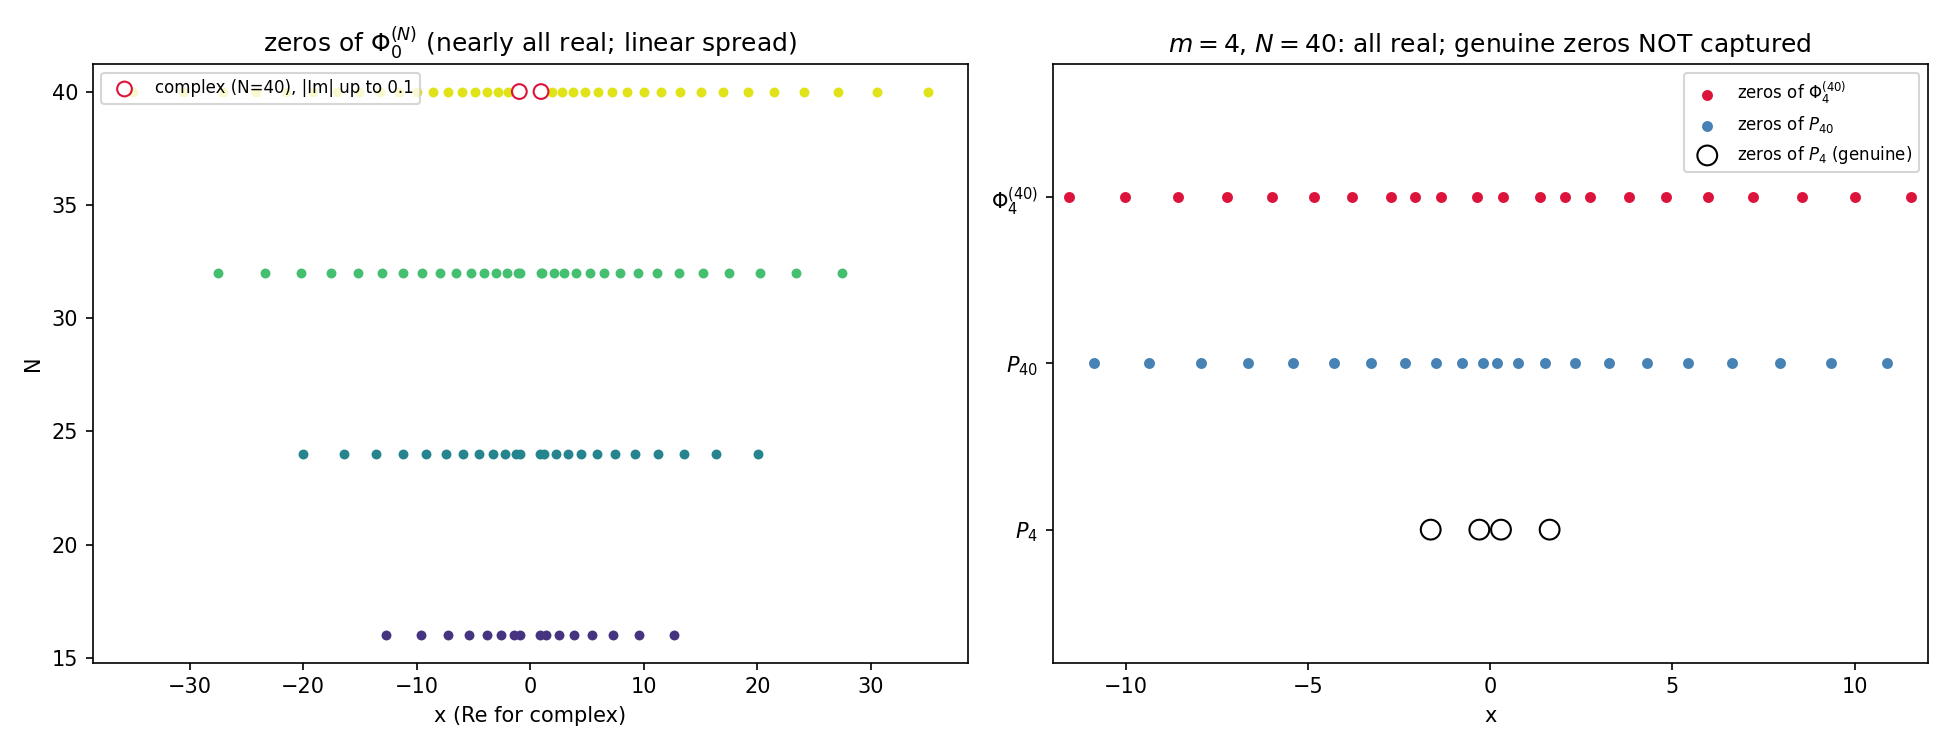
\includegraphics[width=\textwidth]{mp_approximant_zeros.png}
\caption{Left: zeros of $\Phi_0^{(N)}$ for $N = 16, 24, 32, 40$
(all real except four at $N=40$, open circles), spreading linearly
with $N$. Right: the $40$ real zeros of $\Phi_4^{(40)}$ (top row)
against the zeros of $P_{40}$ (middle) and the genuine zeros of $P_4$
(bottom), restricted to $|x| \le 12$.}
\label{fig:zeros}
\end{figure}

%% ===================================================================
\section{Discussion}
%% ===================================================================

The practical consequence for the zeta programme: any function carrying
the archimedean factor $\Gamma(s/2)$ --- including $\xi$ itself on the
critical line --- admits only \emph{algebraic-rate} approximation by
Meixner--Pollaczek polynomials. This quantifies the earlier numerical
finding that the degree-$60$ polynomial approximation of $\Xi$ captures
two Riemann zeros while the Hermite-function \emph{sections} (which
carry the weight-root along and suffer no branch-point mismatch)
capture five or more. In the trade between polynomial bases and
function bases, the $\Gamma$-factor's pole at $s = 0$ --- equivalently
the branch point of $\sqrt{W}$ at $x = i/4$ --- is the entire cost.

Open questions: the exact decay exponent $\alpha$; the large-$k$
factorisation $b_{mk} \sim f(m)\, g(k)$ suggested by the near-rank-one
look of the far off-diagonal entries; and whether the $\lambda = 1/4$
and $\lambda = 3/4$ blocks (even and odd Hermite functions under
Mellin) interact through the joint weight, which the reflection formula
evaluates in closed form:
$|\Gamma(\tfrac14+ix)|^2\, |\Gamma(\tfrac34+ix)|^2 = 2\pi^2 /
\cosh(2\pi x)$.

\end{document}
